% Shared preamble for the repository diagrams. Each figure is compiled twice by build.sh: once as is
% (light theme) and once with \darktheme defined, which swaps the palette for a dark background.
\documentclass[tikz,border=4pt]{standalone}
\usepackage[T1]{fontenc}
\usepackage{lmodern}
\renewcommand{\familydefault}{\sfdefault}
\usepackage{amsmath,amssymb}
\usepackage{sansmath}
\sansmath
% Narrow boxes read better with whole words than with hyphenated ones.
\hyphenpenalty=10000
\exhyphenpenalty=10000
\usetikzlibrary{arrows.meta,positioning,calc,shapes.misc}

% Fill colors encode the role of a step: amber = test or rule, teal = forward simulation,
% purple = optimization or candidate generation, green = state or returned action, red = adverse
% outcome, blue = other processing.
\ifdefined\darktheme
  \definecolor{ink}{HTML}{E6EDF3}
  \definecolor{edge}{HTML}{8B949E}
  \definecolor{blue}{HTML}{1B2E45}
  \definecolor{teal}{HTML}{153C39}
  \definecolor{green}{HTML}{1C3823}
  \definecolor{amber}{HTML}{3F3313}
  \definecolor{red}{HTML}{442022}
  \definecolor{purple}{HTML}{30264A}
  \definecolor{grey}{HTML}{262B30}
  \definecolor{yes}{HTML}{56D364}
  \definecolor{no}{HTML}{F47067}
\else
  \definecolor{ink}{HTML}{17202A}
  \definecolor{edge}{HTML}{5D6670}
  \definecolor{blue}{HTML}{DDEBF7}
  \definecolor{teal}{HTML}{DDF2EF}
  \definecolor{green}{HTML}{E4F2E5}
  \definecolor{amber}{HTML}{FFF0CC}
  \definecolor{red}{HTML}{F8DDDD}
  \definecolor{purple}{HTML}{EAE2F5}
  \definecolor{grey}{HTML}{ECEFF1}
  \definecolor{yes}{HTML}{236B3B}
  \definecolor{no}{HTML}{A33636}
\fi

\tikzset{
  every picture/.style={color=ink, font=\small},
  box/.style={draw=edge, rounded corners=3pt, align=center, inner sep=4pt,
              text width=#1, minimum height=12mm, text=ink},
  box/.default=2.7cm,
  proc/.style={box=#1, fill=blue},   proc/.default=2.7cm,
  sim/.style={box=#1, fill=teal},    sim/.default=2.7cm,
  opt/.style={box=#1, fill=purple},  opt/.default=2.7cm,
  out/.style={box=#1, fill=green},   out/.default=2.7cm,
  bad/.style={box=#1, fill=red},     bad/.default=2.7cm,
  rule/.style={box=#1, fill=amber},  rule/.default=2.7cm,
  ask/.style={box=#1, fill=amber, chamfered rectangle, chamfered rectangle xsep=2pt,
              rounded corners=0pt, line width=0.6pt},
  ask/.default=2.7cm,
  arr/.style={-{Latex[length=2mm]}, semithick, draw=edge},
  darr/.style={arr, dashed},
  lab/.style={font=\scriptsize\bfseries, inner sep=1.5pt},
  ylab/.style={lab, text=yes}, nlab/.style={lab, text=no},
  note/.style={font=\scriptsize, text=ink, align=center},
}

\begin{document}
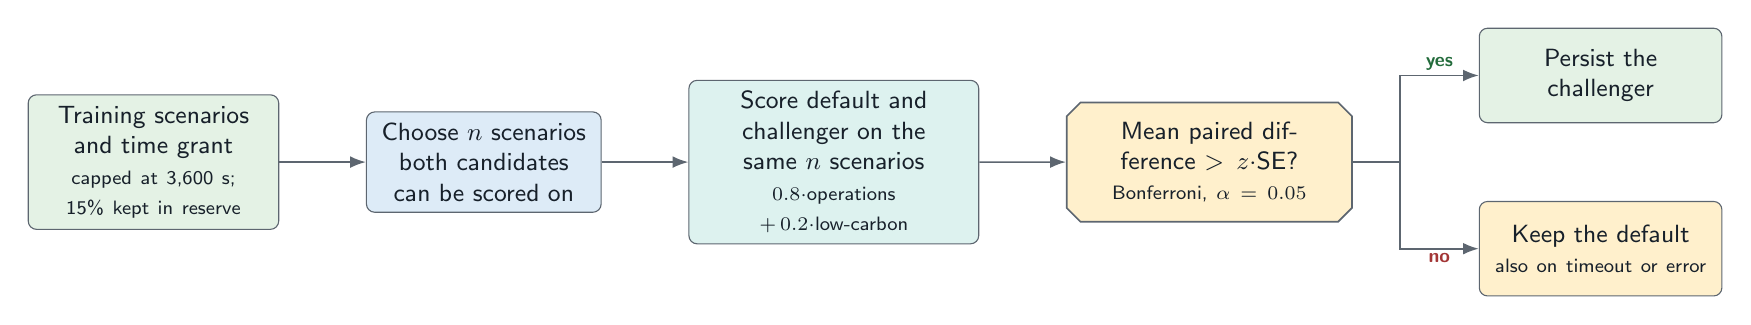
\begin{tikzpicture}[node distance=7mm and 11mm]
\node[out=2.9cm] (g) {Training scenarios and time grant\\\scriptsize capped at 3,600 s; 15\% kept in reserve};
\node[proc, right=of g] (n) {Choose $n$ scenarios both candidates can be scored on};
\node[sim=3.4cm, right=of n] (s) {Score default and challenger on the same $n$ scenarios\\\scriptsize $0.8\cdot$operations $+\,0.2\cdot$low-carbon};
\node[ask=3.2cm, right=of s] (d) {Mean paired difference $>z\cdot$SE?\\\scriptsize Bonferroni, $\alpha=0.05$};
\node[out=2.8cm, right=16mm of d, yshift=11mm] (w) {Persist the challenger};
\node[rule=2.8cm, right=16mm of d, yshift=-11mm] (k) {Keep the default\\\scriptsize also on timeout or error};
\draw[arr] (g)--(n); \draw[arr] (n)--(s); \draw[arr] (s)--(d);
\draw[arr] (d.east) -- ++(6mm,0) |- node[ylab,above,pos=0.75]{yes} (w.west);
\draw[arr] (d.east) -- ++(6mm,0) |- node[nlab,below,pos=0.75]{no} (k.west);
\lanemap{2}{zoom: revalidation in \texttt{train()}}
\end{tikzpicture}
\end{document}
